\documentclass{article}
\usepackage[left=2cm, right=2cm, top=2cm]{geometry}
\usepackage[utf8]{inputenc}
\usepackage{graphicx}
\usepackage{flafter}
\graphicspath{ {images/} }


\title{Mobile Applications Design Document}
\author{Michael Kidd - G00236920}
\date{September 2018} 

\begin{document} 

\maketitle
\clearpage

\tableofcontents
\clearpage 

\section{Introduction}
Create a design and storyboard for a game.  This is a 2D game to be developed as part of the module requirements.  The types of game that are acceptable to design are: 

\begin{itemize}
  \item Shooters – Classic, horizontal or vertical scrolling 
  \item Platform – Classic or 2D 
  \item Puzzle – Action Puzzle or Desktop Puzzle 
  \item Traditional Game – Board Games 
\end{itemize}

We need to research these game types before deciding which design to use.  We must Look at examples of the game types and understand what makes them popular to different players.  Bear in mind that “clone and tweak” is a valid design method in which we pick an existing game and then modify the game world to suit your design. We may design from first principles. 
If we are taking the “clone and tweak” approach, we need to identify clearly the game or games we are using as basis and present the evidence of the type of game it is within the options provided.   \newline
 
For the design, we need to create the following components 
Front End: A term applied to all menus and screens that occur outside of the gameplay.  This takes the player from the title screen to the point that gameplay begins. 

\begin{itemize}
	\item In-Game Menus: A set of menus and screens accessed in-game, often from a pause menu.  These form part of the game mechanisms rather than being distinctly separate. 
	\item Control Mechanisms: The way in which the player controls the game entities.  Many games have just one control mechanism.
	\item The Game: The gameplay screens showing the initial setup, how the action starts, a midpoint in play and the winning/progression conditions depending on the game you are designing.  If the game is episodic in nature, then explain how episodes are defined and how the player moves between them. 
\end{itemize}

\clearpage

\section{Gamer Personality types}
\subsection{Analysts}


\begin{table}[htp]
\begin{tabular}{|l|l|l|l|l|l|}
\hline
\textbf{Game Type} & \textbf{Architects} & \textbf{Logicians} & \textbf{Commanders} & \textbf{Debaters} & \textbf{Overall Average} \\ \hline
\textbf{Sports and racing games} &2.61           &1.99           &5.63           &5.38           &5.24           \\ \hline
\textbf{First-person shooters} &9.66           &10.38           &9.86           &10.77           &12.02           \\ \hline
\textbf{Role-playing games} &35.77           &39.74           &14.08           &36.92           &34.04           \\ \hline
\textbf{Strategy games} &36.55           &28.04           &      47.89     &32.31           &28.67           \\ \hline
\textbf{Stealth-based games} &3.66           &4.19           &5.63           &3.85          &4.25           \\ \hline
\textbf{Card games} &1.83           &1.55           &         1.41  &3.08           &3.81           \\ \hline
\textbf{Other} &9.92           &14.13           & 15.49          &7.69           &11.98           \\ \hline
\end{tabular}
\end{table}

\subsubsection{Architects}
The boundless possibilities of video games that are so often circumscribed by limits of processing power, commercial dictates, or simple imagination may make many Architects at turns frustrated and enthralled. Of the Analysts, Architects may be quickest to go from game play to game design, so confident are they in their ability to improve on the (in their mind) irreparably flawed designs of others.

Even when not making their own creations, Architects may be particularly drawn to game types that allow for a vast amount of control, on both a broad and minute level. Where many more action-oriented games are likely to strike them as hopelessly shallow, strategy and simulation games are probably the biggest draws for Architects. As their name implies, Architects are builders by nature, and they may derive immense satisfaction from games such as the SimCity, Civilization, or Europa Universalis game series, or other so-called “god games” that give them relatively free rein over their dominions. Out of all personality types, Architects took the second place when asked whether they enjoyed strategy games most, yielding only to Commanders.
\subsubsection{Logicians}
Much like Architects, Logicians may be so intrigued by the idea of making their own game that they leave the creations of others behind. However, while Logicians may become briefly infatuated with their ideas, they may not have the resolve to see them through to completion.

Instead, Logicians may content themselves with becoming totally immersed in the systems of a particular game, especially those that allow them to make sweeping, fundamental alterations to the world that is given them. What titles such as Minecraft or Dwarf Fortress may lack in flashy graphics, they more than make up for in their ability to fulfill the restless, voracious imaginations that Logicians possess.

In one of our surveys, Logicians were revealed to be the personality type most likely to “prefer exploring unfamiliar places alone,” and it may be this quality that best explains their gaming preferences as well. Where many games offer prepackaged, predetermined experiences for players to consume, Logicians are rarely satisfied with simply having someone else’s idea of “fun.” Instead, they must forge their own path, accepting the tedious dead-ends that arise as the price one pays in exchange for a happiness that is unshared, and entirely one’s own.

This desire for freedom and independence is clearly reflected in Logicians’ preference for unrestricted, open-world environments – a stunning 84% of Logicians said so in our survey, the highest percentage of all personality types. If you spot someone wandering around a faraway cave in the outer edges of Skyrim, or spending weeks building a medieval castle in Minecraft, chances are you have met a Logician.
\subsubsection{Commanders}
If Commanders are occasionally accused of seeing other people as pawns, it is only because they see everything in terms of chess, where no movement should be made without a careful analysis of the relative merits of all alternatives. And if they view real life through this lens, one can only imagine their ferocity as opponents in virtual spaces. These unchallenged masters of strategy games and attacking roles (the first position in both categories) are a sight to behold, when they get serious about gaming.
\subsubsection{Debaters}
The natural strength of Debaters – their gift for argument – may be largely useless in many video game settings, due to technical limitations making decisions much more binary in nature than the shades of gray that a Debater tends to embrace. And while they may overlook these restrictions in many games, Debaters may chafe more than most at rules when they are at their most arbitrary. Scoring nearly 20 percentage points above average for question “When playing a game, do you engage in behaviors that would be frowned upon in real life, e.g. stealing, tricking other players, breaking alliances etc.?”, Debaters may not be the most reliable allies or treasurers, but they certainly know how to fight their virtual corner and make the best out of any situation.
\subsection{Diplomats}

\begin{table}[htp]
\begin{tabular}{|l|l|l|l|l|l|}
\hline
\textbf{Game Type} & \textbf{Advocates} & \textbf{Mediators} & \textbf{Protagonists} & \textbf{Campaigners} & \textbf{Overall Average} \\ \hline
\textbf{Sports and racing games} &2.07           &1.61           &4.17           &4.13           &5.24           \\ \hline
\textbf{First-person shooters} &6.80          &7.13 &          12.50 &12.39           &12.02           \\ \hline
\textbf{Role-playing games} &48.52           &50.11           &37.50           &40.37           &34.04           \\ \hline
\textbf{Strategy games} &26.04           &20.46          &          26.04 & 30.28          &28.67           \\ \hline
\textbf{Stealth-based games} &2.37           &3.68           &4.17           &0.92           &4.25           \\ \hline
\textbf{Card games} &3.55           & 2.07          &          7.29 &1.83           &3.81           \\ \hline
\textbf{Other} &10.65           &14.94           &          8.33 & 10.09          &11.98           \\ \hline
\end{tabular}
\end{table}

\subsubsection{Advocates}
The world that Advocates envision and the world as it actually exists are often two very different places, and the escapist fantasies that video games offer may therefore be incredibly tempting for this personality type. An Advocate who faces seemingly insurmountable obstacles to their idealism in real life may be pleased beyond words at the relative ease with which such difficulties can be overcome in a digital realm.

As such, Advocates may most enjoy role-playing games with a suitably epic sweep, games such as the Final Fantasy, Dragon Age, or Elder Scrolls series. Aside from loving the notion of being able to “save the world” in a much more clear-cut manner than they are used to, Advocates may also appreciate the sense of personal growth – better attributes, better equipment, better alliances – that role-playing games offer, which appeals to the Advocate’s own perfectionist streak. Sure enough, this is also confirmed by hard data from our survey, with 48.52% of Advocate respondents picking role-playing games as their favorite.
\subsubsection{Mediators}
Perhaps the most conflict-averse of all the personality types, Mediators may prefer playing games solo, disliking the elements of competition that can creep into even ostensibly cooperative game modes. Indeed, their passion for games may be found most in those elements that are the least “game-like,” seeking out titles with fully-realized characters and engrossing stories rather than those that reward lightning-fast reflexes or the ability to sift through reams of statistical data. As the type most likely to see “nothing wrong with avoiding confrontation,” Mediators may seek out gaming environments that are as non-confrontational as possible.

Adventure games – from point-and-click classics like those once produced by game developers Sierra (series like King’s Quest, Space Quest, Gabriel Knight) and LucasArts (series such as Monkey Island, Maniac Mansion, or Indiana Jones) to their spiritual descendants currently being published by Telltale Games (Minecraft: Story Mode, The Wolf Among Us, The Walking Dead) – may be ideally suited for Mediators, who may love nothing more than an opportunity to step inside the worlds depicted therein, without the added pressure of fending off waves of enemies to serve as a distraction. As a rare personality type, Mediators may be accustomed to being outside of the mainstream, and while adventure games have been declared dead countless times over the years, their fan base, small but ardent, has managed to keep them from becoming extinct.

Role-playing games are also likely to be a firm favourite for many Mediators. In our survey, they were the most likely type to pick this genre as their favorite. True wanderers at heart, Mediators strongly agreed that that it is the open-world, exploration-focused games that fascinate them most, taking the first spot among all personality types. They know that straying off a well-travelled path may not necessarily help them complete a quest faster, but is that checkbox in the character log really more important than stumbling upon an interesting side quest or simply stopping by to admire gorgeous scenery? A great story or the well-crafted game world may even cause Mediators to overlook the more tedious (to them) aspects of level grinding and wealth accumulation that are part and parcel of many role-playing games.
\subsubsection{Protagonists}
If Protagonists find themselves fitting easily into the role of hero, they – unlike more Introverted types – may feel that, without an audience for their feats, or compatriots to share their struggle, a game can’t help but feel a bit hollow. They may be as amazed by the beauty, the wonder, and the glory of a richly detailed role-playing setting as an Advocate or a Mediator, but the absence of other living players in an offline game may be a deal breaker for Protagonist Fortunately, there is now a vast array of online role-playing games for Protagonists to dive into, including such favourites as World of Warcraft, Star Wars: Knights of the Old Republic, and Dungeons and Dragons Online. Whether a Protagonist works to build a guild from the ground up or simply basks in the adulation of being the savior of a party, the endless possibilities that these worlds contain may make Protagonists not only play a particular online role-playing game – they may forsake all other games to spend more time with their coterie of online companions.
\subsubsection{Campaigners}
Like most personality types, Campaigners are likely to choose single-player games over multiplayer ones, but they do so significantly less eagerly compared to other Diplomats. It may be that this is more of a necessity than natural preference – like already mentioned above, many great role-playing games, the bread and butter of Diplomat gamers, simply do not have a multiplayer component.
\subsection{Sentinels}
Campaigners also tend to diverge from the rest of the Diplomats when it comes to other aspects of gaming. Perhaps most surprisingly, people with this personality type pick strategy games as their second favorite, even beating one Analyst type, the Logician. One may argue that many strategy games reward improvisation and ability to think on your feet, key strengths of the Campaigner. Still, this is a rather surprising discovery.

\begin{table}[htp]
\begin{tabular}{|l|l|l|l|l|l|}
\hline
\textbf{Game Type} & \textbf{Logisticians} & \textbf{Defenders} & \textbf{Executives} & \textbf{Consuls} & \textbf{Overall Average} \\ \hline
\textbf{Sports and racing games} &2.89           &2.48           &5.14           &7.43           &4.49           \\ \hline
\textbf{First-person shooters} & 10.13          &8.56           & 9.88          &13.71           &10.57           \\ \hline
\textbf{Role-playing games} &36.16           &46.55           &34.78           &28           & 36.27          \\ \hline
\textbf{Strategy games} &33.08           & 24.66          &          27.27 &26.86           & 27.97          \\ \hline
\textbf{Stealth-based games} & 4.05          & 2.76          &  2.77         &6.29           &3.97           \\ \hline
\textbf{Card games} &1.83           & 2.94          &          5.53 & 4          & 3.58          \\ \hline
\textbf{Other} &11.86           &12.05           &         14.62 &  13.71         &  13.06         \\ \hline
\end{tabular}
\end{table}

\subsubsection{Logisticians}
When the abstract messiness of the world gets to be too much for a Logistician, they may find themselves reaching for a game with finite, concrete rules, one that is easy to learn but difficult to master. Logisticians are not likely to invest a great deal of their time in these games – lest they turn into efficiency-sapping time sinks – so those which have lengthy tutorials or extensive narratives will probably not receive a second glance. While people with this personality type are not the most likely to see gaming as a waste of time, they are not particularly enthusiastic about such activities either, landing close to the middle of the list when it comes to time spent playing games.
\subsubsection{Defenders}
The utter selflessness of Defenders may cause many to reject gaming on the grounds that they are far too busy taking care of others to indulge in such a frivolous activity themselves. Even as Introverts, the idea of sitting alone with a console game for hours on end may hold absolutely no appeal. This is confirmed by our survey as well, with most Defenders saying that they spend less than 3 hours each week playing games. Even then, most of their gaming sessions would probably happen on their phones – Defenders had the second highest score of all personality types when asked about smartphone gaming.
\subsubsection{Executives}
Of all the personality types, Executives may have the most difficult time engaging in “trivial pursuits,” those activities which have no obvious use but to relax and have fun. Many Executives may see games as a time-wasting vice, not only worthy of ridicule, but actively harmful to one’s personal productivity. Of course, Executives are not immune to the pleasures of video games – however, they may go to great lengths to downplay their own enjoyment, even battling their love of play as one might battle one’s indulgence in alcohol or sweets.

This attitude is quite obvious in our survey as well. Executives are the personality type most likely to spend less than 3 hours per week gaming, and they are also clearly disinterested in professional e-sports, taking the last position both for “Do you watch any games or specific players online, e.g. on Twitch?” and for “Would you like to be a professional gamer?”
\subsubsection{Consuls}
As video gaming has achieved a greater level of acceptance in mainstream society, Consuls have followed suit, although their aversion to appearing “strange” may still lead them to picking up a game only after a sufficient number of their acquaintances have found themselves hooked. And where other personality types may experience little or no embarrassment at being “caught” playing a game for hours on end, Consuls may nurse their passions in secret, casually dismissing the time spent as “only because they wanted to see what all the fuss was about.”

Consuls, then, are likely to prefer those games that are most widely played within their cohort: sports fans may see series like Madden or FIFA as an organic extension of their fandom, for example. Our survey confirms that as well, with Consuls getting the highest score for sports and racing games among Sentinels, and well above the overall average. There may be a certain social factor in play here too, as Consuls are also more likely than other personality types to embrace multiplayer games – perhaps in the form of sitting down with their friends for a FIFA session every once in a while.
\subsection{Explorers}

\begin{table}[htp]
\begin{tabular}{|l|l|l|l|l|l|}
\hline
\textbf{Game Type} & \textbf{Virtuosos} & \textbf{Adventurers} & \textbf{Entrepreneurs} & \textbf{Entertainers} & \textbf{Overall Average} \\ \hline
\textbf{Sports and racing games} &5.56           &          5.45 &15.38           &7.50           &5.24           \\ \hline
\textbf{First-person shooters} &5.56           &10.91           &30.77           &17.50           &12.02           \\ \hline
\textbf{Role-playing games} &38.89           &32.73           &15.38           & 15          &34.04           \\ \hline
\textbf{Strategy games} &29.63          &21.82           &          23.08 &32.50           &28.67           \\ \hline
\textbf{Stealth-based games} &0           &9.09           &          11.54 &7.50           &4.25           \\ \hline
\textbf{Card games} &3.70           &5.45           &          3.85 &2.50           &3.81           \\ \hline
\textbf{Other} &16.67           &14.55           &0           &17.50           &11.98           \\ \hline
\end{tabular}
\end{table}


\subsubsection{Virtuosos}
Virtuosos can at times seem paradoxical to outside observers, combining tough rationality with a childlike sense of wonder, and the ability to become completely absorbed in a project, only to abandon it the moment their interest begins to wane. In many ways, though, this type epitomizes “classic” video games, the type that originated in arcades before making their way into the homes of millions.

Video games like Pac-Man, Donkey Kong, or Asteroids were built around seemingly simple mechanics, but this simplicity was often deceptive, allowing a neophyte to breeze through a few stages before the difficulty became exponentially greater with the tweaking of only a few variables, such as the number, speed, or attack patterns of the enemies one faced. Mastering the skills needed to succeed in such fast-paced environments may be exactly the type of challenge that a Virtuoso craves, whether they stick to the classics or play more contemporary variations like platformer Super Meat Boy or “bullet hell” shoot-em-up Ikaruga.

Judging from our survey, Virtuosos are the personality type that spends the highest number of hours per week playing games – a stunning 70% of respondents said that they do that for more than 3 hours per week, with half of them going over 10 hours. It does indeed seem that the explosion of choices for games has been a real boon for Virtuosos, giving them an opportunity to apply their skills and abilities in virtual worlds.
\subsubsection{Adventurers}
Although “adventure” would seem to be an integral part of the gaming experience, the borders of many games are all too easy to encounter for the Adventurer. Whether hemmed in by linear narratives or restrictive environments, Adventurers have little desire to simply replicate the movements that a designer has dictated for them to follow.

For Adventurers, the “sandbox” style of games have been an absolute boon, although they may prefer those that emphasize spontaneity and cosmetic customization rather than long-range planning and tweaks made on a more molecular level. Perhaps first popularized by the Grand Theft Auto series, open world action games are now practically a genre unto themselves, from Saint’s Row to Just Cause to many more titles with greater or lesser degrees of flexibility in play.

It is no surprise then that in our survey, Adventurers were the most likely personality type to pick PC as their favorite gaming platform, with 63.64% of respondents saying so. PC gamers do indeed have a plethora of options to choose from when it comes to “sandbox” style gaming. Adventurers also scored above the overall average when asked whether they enjoyed open-world games, reaffirming our statements above.
\subsubsection{Entrepreneurs}
Thrill-seekers and daredevils who win followers through their quick thinking and sheer gutsiness, Entrepreneurs can be a tough crowd for many games, often growing bored before the menu screen has had time to finish loading. The games that hold their attention usually must be both intensely fast-paced, yet accessible enough not to demand dozens of hours to achieve a baseline competence.

Multiplayer shooters, such as the Call of Duty, Battlefield, or Halo game series, are perfect for Entrepreneurs, who may drop into a game for a couple of hours of frenetic action with little setup time, and drop out again the moment their focus beings to waver. The most competitive of Explorer types – and among the most competitive of all the personality types – Entrepreneurs may not grieve over their losses for long, but during a game, few can hope to match their intensity.

It is not a surprise then that Entrepreneurs have the third highest score for console gaming and they are also unmatched proponents of both first-person shooters and sports and racing games, scoring more than twice as high as the overall average in both categories. While there may be a rare Entrepreneur willing to pour days into an epic Civilization V game, an hour with the latest Call of Duty or Need for Speed release is more likely to attract someone with this personality type.
\subsubsection{Entertainers}
“Single player only” is a phrase that is not in an Entertainer’s gaming vocabulary, and even many multiplayer games may not have what it takes to arouse their interest. For example, the team-oriented play of squad-level shooters or online role-playing games may not allow for enough opportunities for their star to shine. In our survey, Entertainers landed firmly on the multiplayer side, nearly 20 percentage points above overall average and second among all personality types.
\clearpage

\section{Game Design Research}

\subsection{Shooter Games}

\subsubsection{Defender(1981)}

\begin{minipage}{0.4\textwidth}
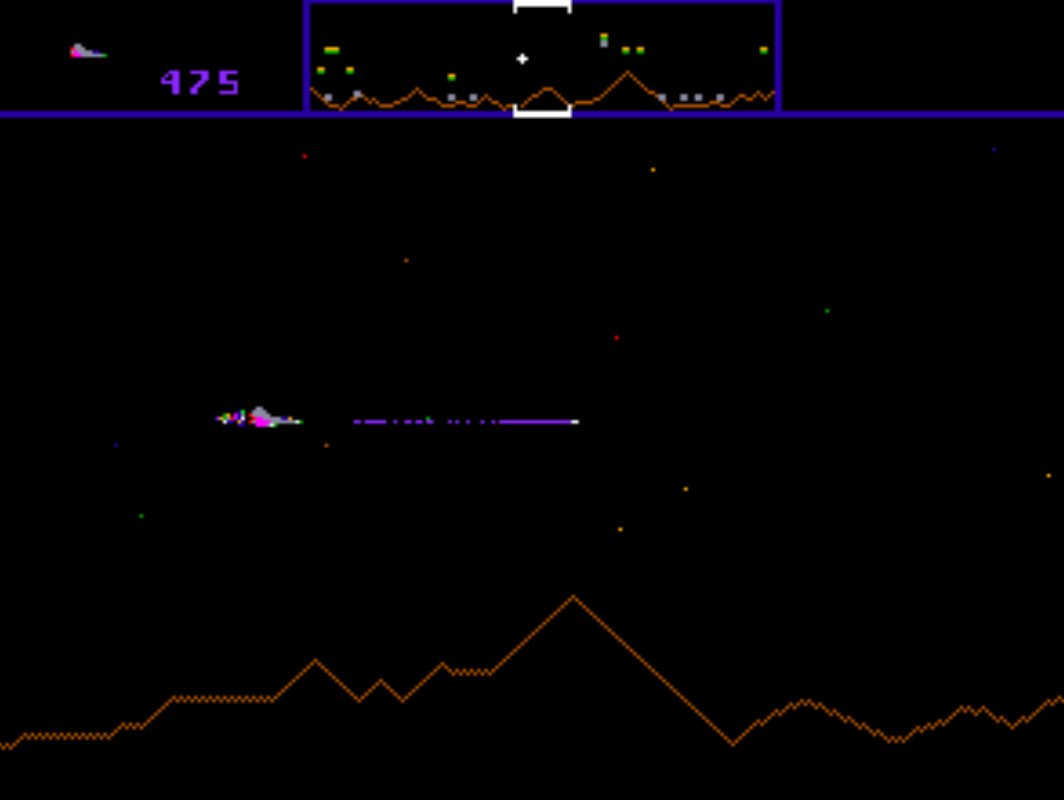
\includegraphics[width=\linewidth]{defender}
\end{minipage} \hfill
\begin{minipage}{0.55\textwidth}\raggedright
Defender is a 2D Side scrolling shooter, the controls were simple compared to today's style of games and control schemes, of course this didn't make the game any less difficult. \newline \newline
The game was designed by Williams, an American company that originally was a creator of pinball machines, like many other arcade video games.
Williams had failed already to make an imitation game of the now home console classic Pong by Atari, which itself was an accidental imitation of the game that came with the Magnavox Home console. Defender was their first big arcade game. It was one of, if not the first side scrolling  games that was later perfected by Super Mario Bros. The game made more than 1 billion US dollars. \newline
\end{minipage} \newline \newline

The most memorable High score for Defender was from Steve Jurassic who scored over 23 million points in Iowa. Due to a query by Walter Day, the owner of twin galaxies which at the time was a video game arcade, to find out if this score was the highest in defender. When Walter had queried the score, realising that nobody knew the answer, then decided that he would start Twin Galaxies and gather high score for arcade video games. This later led to the many video game controversies and stories regarding high scores on games such as Donkey Kong, Pacman and Berserk. \newline

Defender was set on a black backdrop as many games did at the time. Many games of this generation were copies or imitations of the game Space Invaders. Space invaders was a single screen shooter were the players avatar was shown at the bottom of the screen, it was able to move back and forth and shoot at alien ships that would be progressing down the screen. The player was tasked with shooting the alien ships before they reach earth. With defender the difference was that the game side scrolled, the players ship would traverse a level by moving up, down, left and right. Were Space Invaders and its multiple clones were simple shoot em ups, Defender took the approach of making the players run defend and rescue missions. The Creator Eugene Jarvis stated that he came up with idea for the game from the title of the 1960's TV show the Defenders, which was a court room drama that Jarvis loved at the time. He also stated that when you are defending from an enemy you can do what you want. One of the fun facts about with the game was a bug that happened when a player would reach the score of 990,000, the player would receive a boost in smart bombs and extra lives, even though it was a bug the creator stated that it was part of the fun of the game.
\clearpage	
		
\subsection{Platform Games}

\subsubsection{Donkey Kong(1981)}

\begin{minipage}{0.4\textwidth}
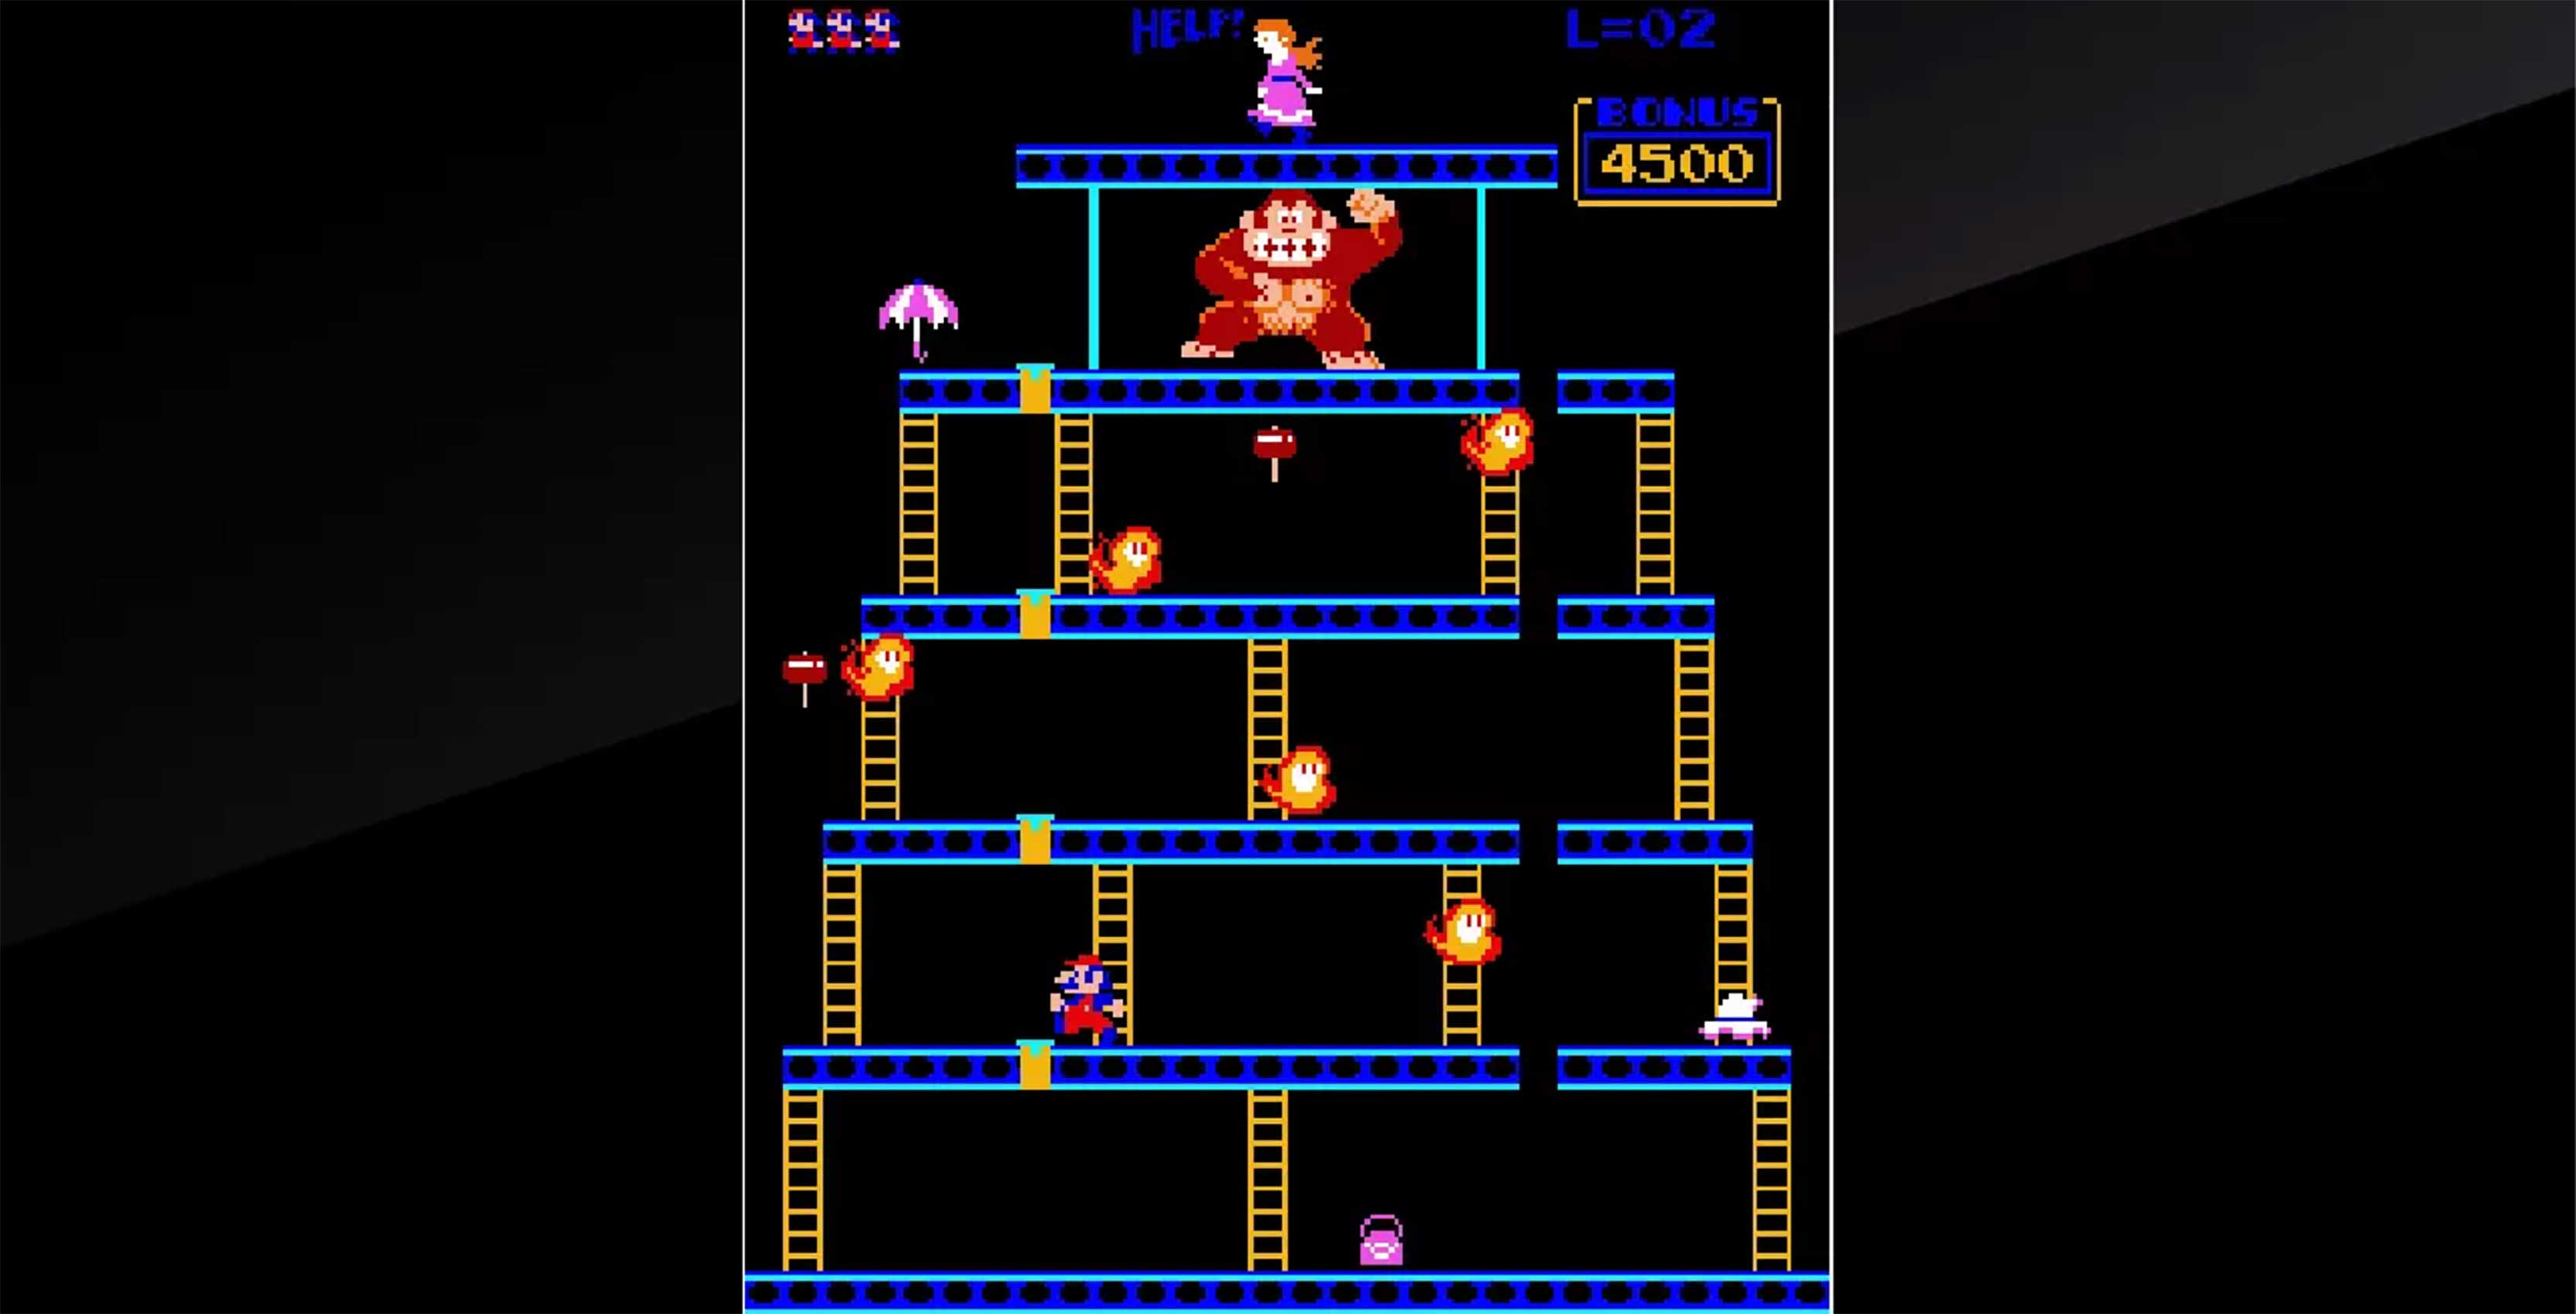
\includegraphics[width=\linewidth]{donkeykong}
\end{minipage} \hfill
\begin{minipage}{0.55\textwidth}\raggedright
Donkey Kong was released in 1981 by Nintendo, The game was the first Mario game but at that time he was known as Jump man, it consisted of Mario starting at the bottom of a number of ladder stages, while Donkey Kong, a large ape at the top, would throw barrels and objects that would role through the platforms. The goal was to get mario to the top of the stage and get to the awaiting princess and then Donkey Kong would steal the princess away and the game would progress to the next stage. The game is incredibly difficult, with most gamers failing the first few levels due to the random nature of the obstacles and events, such as barrel, fireball and spring volume.
\end{minipage} \newline

Donkey Kong himself was based on the Kong character from the 1933 film "Kong". Although Universal studios had attempted to sue Nintendo for infringement, Universal studios had already in a previous case stated that Kong and its story were public domain, meaning that Universal had no legal claim for infringement. Like many arcade games at the time, there was not an end level to the game. The game would simply run out of memory and would result in what was known at the time as a "kill screen". In Donkey Kong the kill screen resulted in the game freezing on the final stage and mario would begin to spin and the game would finish. Whatever score you had at this point would be your final score, however only the best players would ever get to this point. The arcade industry relied on people playing games and putting money into the machines, so a pro player who could put in one coin and play for a day or two for a handful of coins was not financially beneficial unless that player could draw a crowd to the arcade. \newline 

 Billy Mitchell who was the top scorer in the game centipede, while appearing at an event for life magazine took the high score for Donkey Kong in 1982, with a score of 874,300 in just one run. Beating the previous record holder by more than 300,000 points. He later became a record holder for the first perfect game in Pacman, this meant he finished 256 levels in pacman and eliminated each ghost in those levels in one life, if you ever played Pacman, you will know how hard that is to accomplish. \newline \newline
After years of controversy Billy Mitchells scores were removed from Twin Galaxies and the Book of Guinness world records after it was discovered that the tapes of his record were filmed using an emulator, not an official arcade machine. This means that all of his previous scores have also been removed and makes Robbie Lakeman the highest score in Donkey Kong which was acheived in February 2018. Billy Mitchels Score stood for 25 years until it was broken by Steve Wiebe, who originally was the first person to break 1 million points in the game but Billy Mitchell refused to accept the score as he stated it was not done live, even though Mitchell himself has never been seen setting a score in the game live since his original record. Some of this information and interesting story can be seen in the Documentary "The King of Kong". \newline \newline

In 1994 Nintendo released Donkey Kong Country on the super Nintendo, this game i remember very fondly as it was a big game for me as a kid. This is one of the few games I didn't get in trouble for spending hours playing this at my house, mainly because when this was on everyone at home would gather round to see if I could complete the level and would take turns to try beat the level when I failed. In 1994 we still had CRT televisions and would hurt your eyes with long periods of staring at the screen. Not to mention that if your console was hooked to the only TV in the house, the hours of gaming kids put in today would be difficult as parents or sibling would be queued for the TV. Today you could take a console that fits in your pocket or an iphone and just play a game like this. As of 2018 there is a Donkey Kong game in the same format of Donkey Kong Country on the Nintendo switch. This game is known as "Donkey Kong Tropical Freeze", showing the longevity of Donkey Kong 38 years after its creation and how far it has come from a game that existed inside a box in an arcade and had only 4 levels.
\clearpage

\subsubsection{Super Mario Bros.(1985)}

\begin{minipage}{0.43\textwidth}
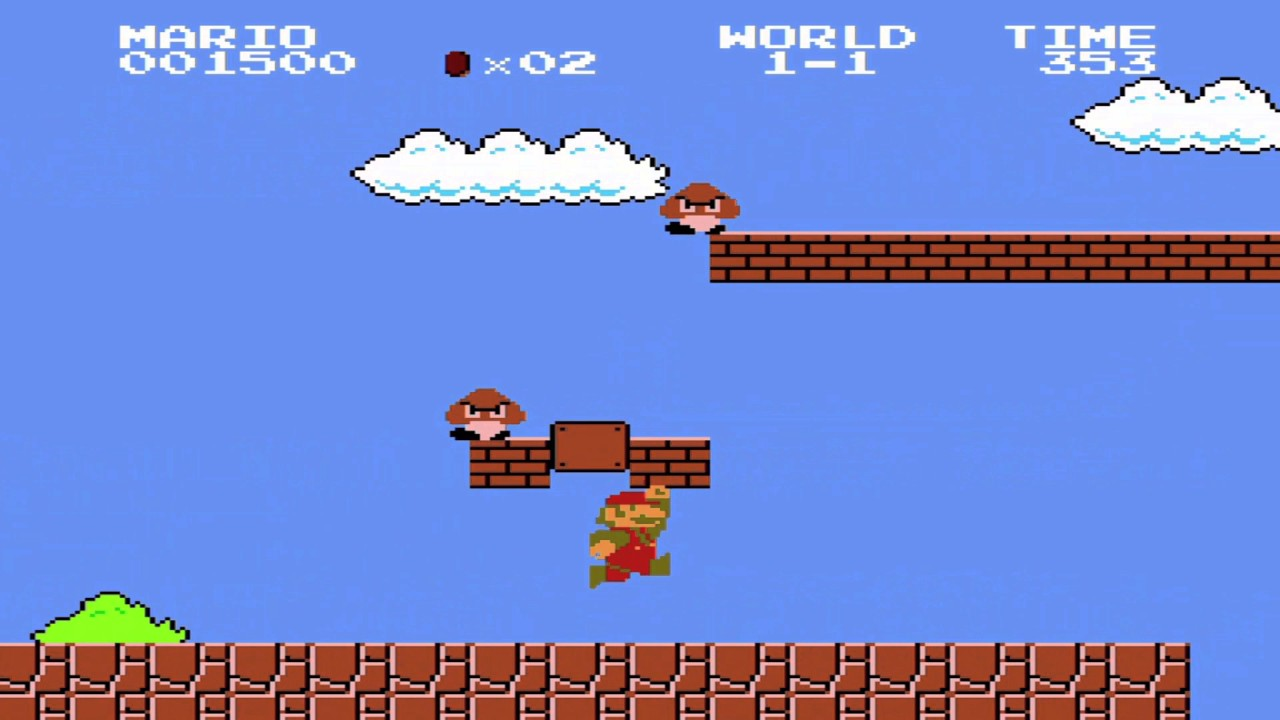
\includegraphics[width=\linewidth]{mario}
\end{minipage} \hfill
\begin{minipage}{0.55\textwidth}\raggedright
As one of the biggest names in gaming history and the face of an empire, that being Nintendo, Mario had his humble beginnings as previously mentioned in the last[[
 section about Donkey Kong. Mario started without the name Mario and was known at the time as Jump Man. In the game Jump Man represented an ape trainer. Donkey Kong escapes his Captor(Mario), Donkey Kong then kidnaps jump man's girlfriend and drops barrels and springs in an attempt to stop the trainer from reaching the top of the platform where he can reach his girlfriend and then Donkey Kong will take her and run to the next level. The game had a huge following and Nintendo decided to give Mario his own story and game.
\end{minipage} \newline 

Nintendo went on to release super Mario Bros in 1985. which went on to sell 63 million copies of that game alone and more than 600 million games in the franchise. The first game was released on the Nintendo entertainment system in 1985. The levels consisted of a side scrolling platform game, when Mario moved the background moved with him. Mario's goal was to rescue princess peach who has been kidnapped by the evil bowser. Mario would have to traverse each level to reach the end, which various degrees of difficulty and different types of obstacles. Each level would also consist of platforms that allowed Mario to navigate the level in a new way, such as avoiding an enemy by jumping to a platform overhead or by travelling down a tube and skipping to a section further up the level. \newline

One of the things that made Super Mario Bros. so popular was its level design, nothing was placed in the game to fill space or to just make the game harder, everything had a purpose. Mario starts out as a small version that if comes in contact with a trap or enemy will loss a life. Mario can become large by eating a mushroom, there is also a blue mushroom that will hurt Mario or make Mario loss a life. You also need to collect coins and with every hundred coins you gain a life, or 1UP as we called it.  Mario could eat a plant and this would allow him to shoot fireballs from his hands to take down enemies. If Mario was injured from either his large state or while having the ability to shoot fire, he would revert back to the small Mario stage. If Mario was to fall through the gaps in the floor he would loss a life also. when all lives are lost the game restarts. This level of difficulty gave the frustration that players who were good at the game needed to get them hooked on the game and the new players could become hooked because the game made sense in how it worked, most people could figure out that the mushroom made   Mario big, or that he couldn't come in contact with an enemy. This would also be obvious to a player without a tutorial level or text on screen to explain it. This meant it did not matter what language you spoke, you would understand this game and it was addictive. \newline 
Shigeru Miyamoto explained during an interview, that he had designed the first level of Mario last. The reason this was done, was because it allowed him to see how people played the inner levels of the game and design the first level around the game play and make the game introduction intuitive and easy to pick up for new users, as this would mainly be a home platform, it was essential that people would watch the screen of a player, understand how the game was played and when they tried it would be able to simply play the game without a verbal explanation of the game, without making the game too easy to complete.  \newline 

Since Mario's creation he has appeared in well over 200 video games across multiple platforms and today is still the flagship game for any Nintendo device whether it be a platform game, a Mario 3D world game or my personal favourite Mario Kart racing games. It is clear that Mario has lasted a long time and has no signs of slowing down, a testimonial to how a plumber with no considerable back story can start an empire and become a gaming icon for generations.
\clearpage		

\subsection{Puzzle Games}

\subsubsection{Tetris(1984)}
\begin{minipage}{0.43\textwidth}
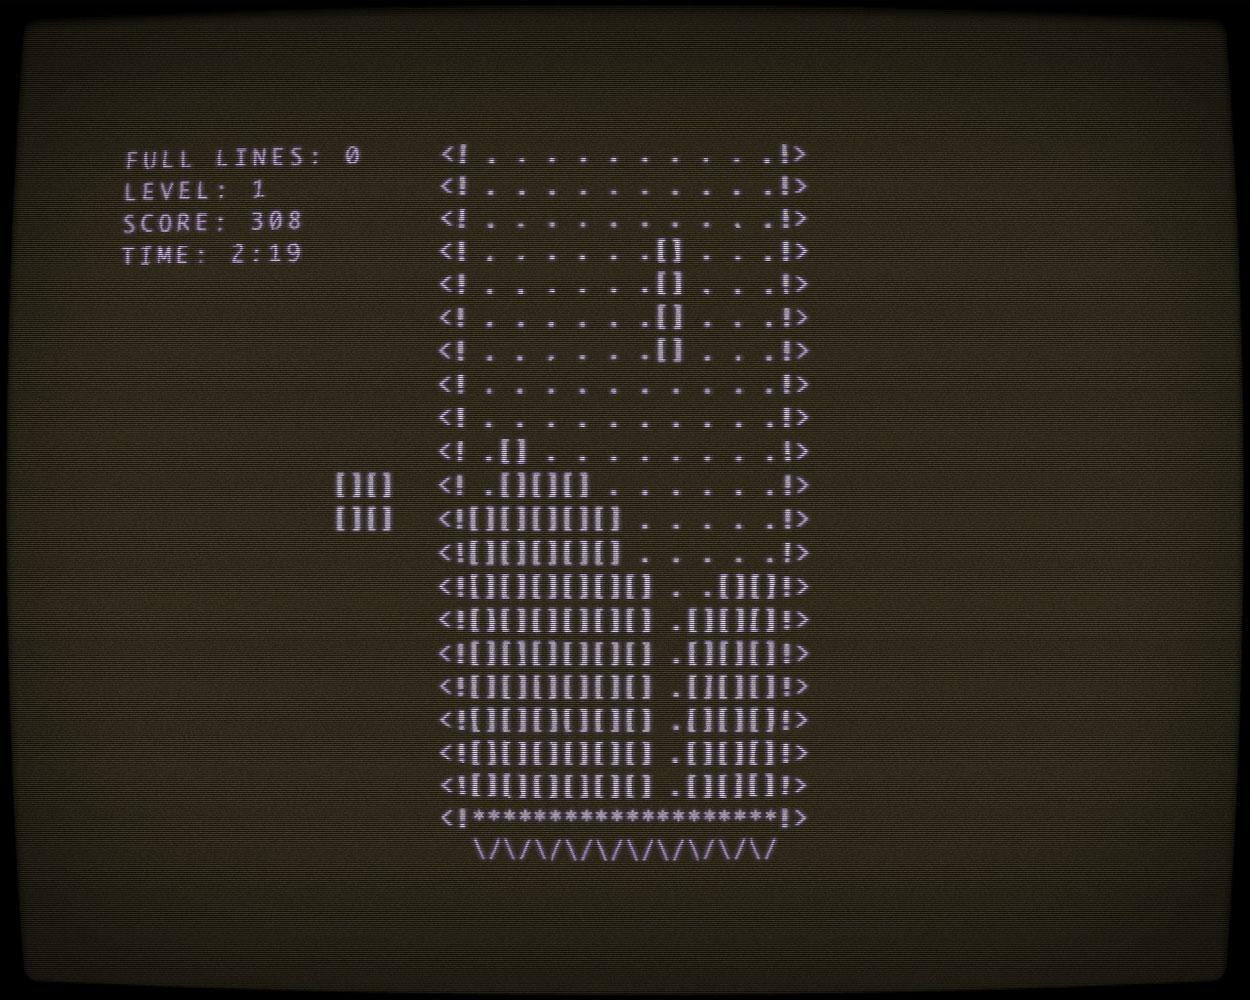
\includegraphics[width=\linewidth]{tetris}
\end{minipage} \hfill
\begin{minipage}{0.55\textwidth}\raggedright
During the cold war in 1984, A young programmer named Alexey Pajitnov created the game we know as Tetris, possibly the greatest puzzle game of all time. The idea was originally a game he called genetic engineering, it had the same shape Tetris has except more like a jigsaw puzzle, the idea was to place the pieces in an order that fill the main box with no pieces left over and no blank spaces. Later her made tetris as we know it now. He made the screen narrower than it was and had the pieces fall and the use could move the pieces across the screen and rotate the pieces so that they we fit better with the pieces already placed. Originally they simply stacked and the game ended when the screen filled. Later he changed it so that when the player filled a line, it would delete the line and increase the players score. This was the step that made the game very popular. \newline
\end{minipage}

The game was named after Tetraminoes, named after the four pieces each of the block were made up of. The game originally started out as share ware, which was common at the time and also common with alot of games and software when i was young. It would be normal to place this type of software onto a floppy disc and pass it to a friend, usually with the intention of setting high scores and testing if you could beat your friends scores. \newline

Tetris beginning as can be imagined was not an easy one, due to the cold war and how the game was created by a programme than worked on the Russian side of the iron curtain. Alexey Pajitnov had created the game at the Russian Academy of Sciences, this made the game the property of the Russian government. Due to the games addictive gameplay, the game quickly spread. It made to the US and was picked up by Robert Stein who had to fight a legal battle for the rights to the game and even had to attend a meeting in Russia to negotiate the sale of the game. The game was then released on the US market by Spectrum Holobyte. \newline

One of the great facts that I enjoy about Tetris on the Nintendo Gameboy system is that Steve Wozniak, the co-founder of Apple Computers was so good at the game that he held the high score for so long and dominated it, that Nintendo banned him from submitting scores. Wozniak then started submitting his scores while spelling his name backwards(Evets Kainzow). The reason that the Gameboy was released with Tetris in place of Mario as expected when Nintendo release a system was from one famous statement from game developer Henk Rogers who said "If you release the gameboy with Mario, it will be for little boys, if you release it with Tetris, It will be for everybody". The highest score on classic NES Tetris is 999,999. If you even get close to that, you are an incredible gamer. The 1987 PC version of Tetris came with a 'boss button'. It pulled up a generic spreadsheet on your screen to make it look like you were working rather than playing a computer game at your desk. \newline

Another interesting fact regarding Tetris, If you have ever played a game so much that you start to dream of the game or had the mental image of the game. This is known as the Tetris effect or Tetris Syndrome, I have experienced this like most gamers, most notably as a teenager I remember playing chess so much, that I was imagining human beings who were speaking in a group as being chess pieces placed on a board. When I was asking people to move from where they were standing was when i knew I should stop playing for a while. \newline
\clearpage

\subsection{Traditional Games}

\subsubsection{BattleChess(1988)}

\begin{minipage}{0.43\textwidth}
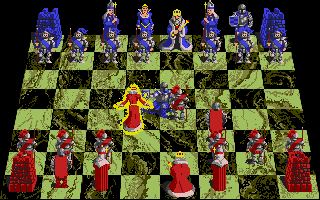
\includegraphics[width=\linewidth]{battlechess}
\end{minipage} \hfill
\begin{minipage}{0.55\textwidth}\raggedright
For this list I wanted to include a traditional tabletop game that was used as a video game, Obviously we have games like poker, UNO and even monopoly that have been brought to the video game world, But there are hundreds, possibly thousands of those with very little variation on the original. Then we have Battle Chess. A game released in 1988 and release on the Amiga, then brought to  3DO Interactive Multiplayer, Acorn Archimedes, Amiga CD32, Amiga CDTV, Apple IIGS, Apple IIe, Atari ST, Commodore 64, MS-DOS, FM Towns, NES, Mac OS, NEC PC-9801, X68000 and Microsoft Windows. Even thought it was obviously successful enough that it has been ported and enhanced to so many systems, this is the one game in the list I find very Irritating and that may be one reason I have chosen to include it. Even as a fan of chess and video game individually I found this game to be unplayable.
\end{minipage} \newline

It did have all the basics of Chess, all the moves are there, No special moves have been added. When a piece takes another piece however, an elaborate animation is played with those pieces fighting and the taken piece losing to the aggressive piece. The problem with this was that it happened every time a piece was taken and even made noises when they moved, so it becomes frustrating quickly. Any serious chess player would probably give up after the first few minutes, when the gimmick wears off. Anyone who was in the game for the animations and little fight animations could have played something better, and if you enjoyed the animations for longer than a game or two and kept playing, then their  must be something wrong with you and you probably went on to create the Postal games. \newline

\subsection{Research Conclusion}

After researching each of the games and history of the golden age of arcade gaming, I have found that Research anything can be boring if done enough, even something you have done your whole life and something I have followed closely since I was a Child. Besides that, I have gained a good insight into what made these games popular and why so many people and myself included spent hours in arcades or glued to a CRT screen everyday, even though our eyes were watery and tired. Even though our parents told us not to and in some cases the other kids made fun of us for it. \newline

The Reason was simple. we loved these games, we loved the challenges. We loved the High scores and trying to beat them, we looked trying to get one more point than we did last time, or beating the guy at the top of leaderboard we never met and could only identify by their 3 initials. All of these games had common traits though. Defender and games like space invades brought ahead the arcade generation were people flocked to arcades to play these games. Donkey Kong showed games could be very addictive while being insanely hard to play, it also brought us Mario, and even though Donkey Kong came first, Everyone knows Mario. Mario hasn't had a real break in the gaming world, Its always doing something. Tetris brought gaming to the work place, so much so that they included a button so you could hide it from your boss. People look today at games like Pokemon Go and see that its on the news, being played by people all over the world. Tetris did that too, but instead of that being downloadable on a smart phone that almost everyone has, It was passed around on a floppy disc, from side of the iron curtain to the other, in a time when it would have caused someone to be executed for passing information across borders. Just so it could be passed around the office on a floppy disc. Thats were games that last forever come from. From addiction, from not knowing when its going to end. Most of the  time for not knowing if you are evening one of the good players of the game or not. 
\clearpage

\section{Design}

\begin{minipage}{0.4\textwidth}
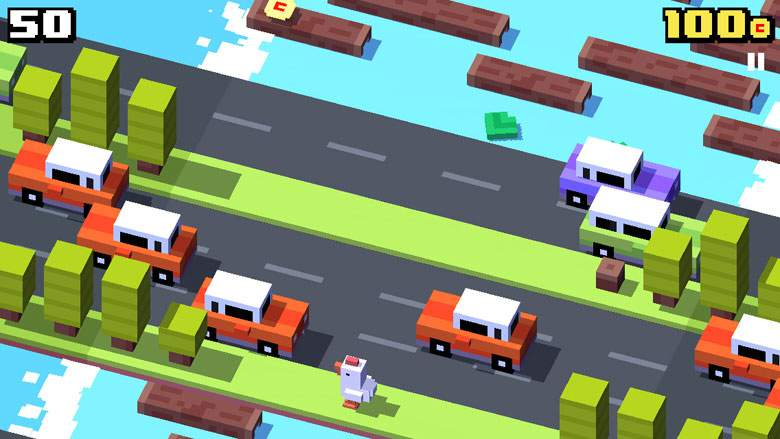
\includegraphics[width=\linewidth]{crossyroad}
\end{minipage} \hfill
\begin{minipage}{0.55\textwidth}\raggedright
The game that I'm going to base my project on is a game called Crossyroad, it has been described as a cross between Frogger and Flappy Bird. The game takes a humorous look at why the chicken crossed the road. You play as a chicken, you can move up and down, but also move forward. the goal is to gain points by staying alive, get the chicken across the road by tapping on the screen and going one grid at a time. The game is an endless runner with a procedurally generated level.
\end{minipage} \newline

This makes the game addictive and different every time you play it. I have been stuck to this game in the past similar to Donkey Kong, In fact myself and my partner would try beat each others scores while the other was asleep. The reigning champ would node off happy in the knowledge that they had a high score the other couldn't beat. Then wake up the next day opposed and have to cancel work to reclaim the title, or simply wake up wondering why the other hadn't slept all night and seemed very irritable. \newline
Crossyroad is a 3D platform endless runner, but i will be making a 2D version. In place of a chicken I will be using a ball that can rotate and force can be added to, this will mean it will be harder to control. The reason that i have chosen this type of game is because of the best ideas from the games I have listed in my research. Kong was addictive due to its random nature and the fact that you still needed a lot of skill and luck to get the high scores. Mario was amazing due to its intricate, well thought out level design that made it easy for a new player to understand the mechanics of the game. Tetris was great because of the possibility of it never ending if only you were good enough to make it happen. Even on a handheld device with no internet connection, you still had yourself to beat and ou are better at the game today than you were yesterday. A game that people played so much they start seeing the game in real life. \newline

\begin{minipage}{0.35\textwidth}
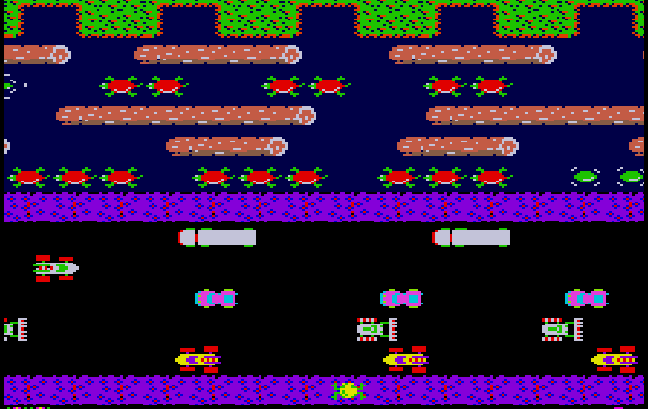
\includegraphics[width=\linewidth]{frogger}
\end{minipage} \hfill
\begin{minipage}{0.55\textwidth}\raggedright
Crossyroad is an imitation of is Frogger. The rules of the game haven't changed much between the two games, but crossyroad is an endless runner and frogger is not, this is why I have made the comparison with crossyroad, as it will be more of a representation of the game that I will make.

\end{minipage} \newline

\subsection{Front End}

The front end of the program will run on the windows platform using UWP and built using Unity. The user will be able to select either a touch screen control or a keyboard control scheme.

\subsection{In-Game Menus}

The first screen the user will be able to see is the login screen, If the user likes they can create an account with a link from this screen.
On the account creation screen, the user can add a user name and must enter a password twice. Then have an option to submit the information to have it verified. As a point there will be no in game pause screen, when the player has failed the level or died, they will be presented with a screen that will ask if they want to restart or quit, along with information about their score, if this is their best score, it will be added to a leader-board that is stored on a Firebase database and they will be shown the top 10 players and their own position in that list.

\begin{minipage}{0.5\textwidth}
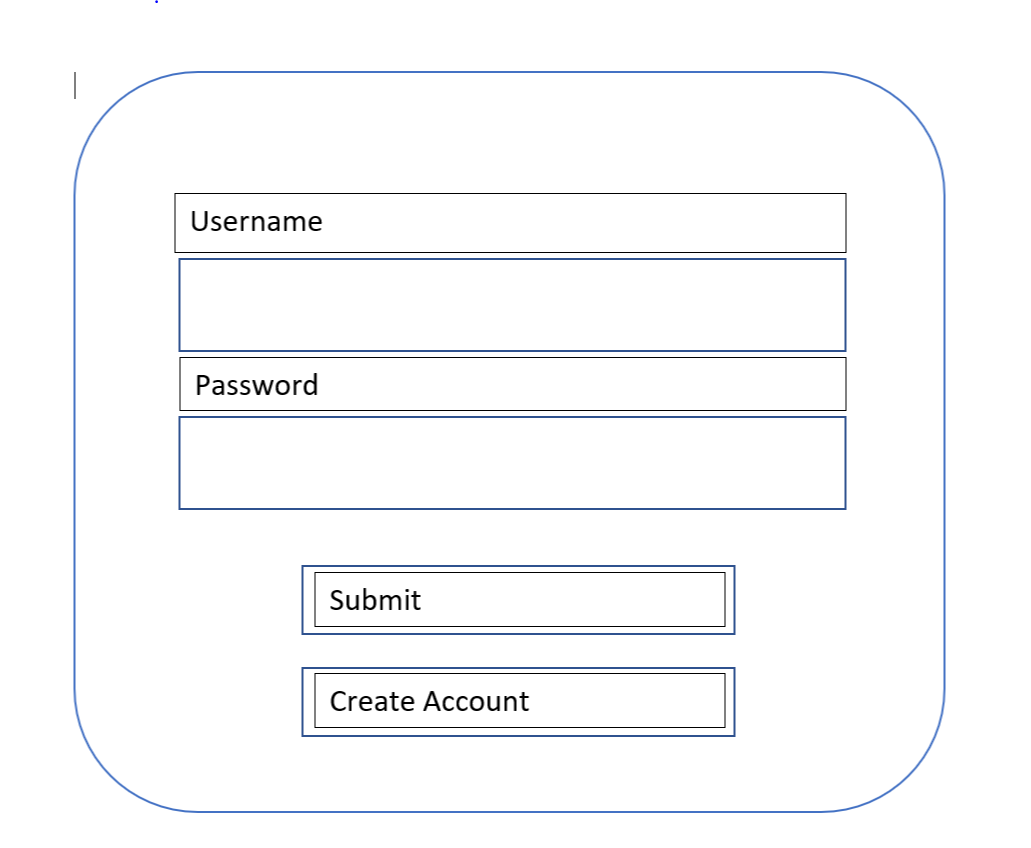
\includegraphics[width=\linewidth]{loginscreen}
\end{minipage} \hfill
\begin{minipage}{0.5\textwidth}
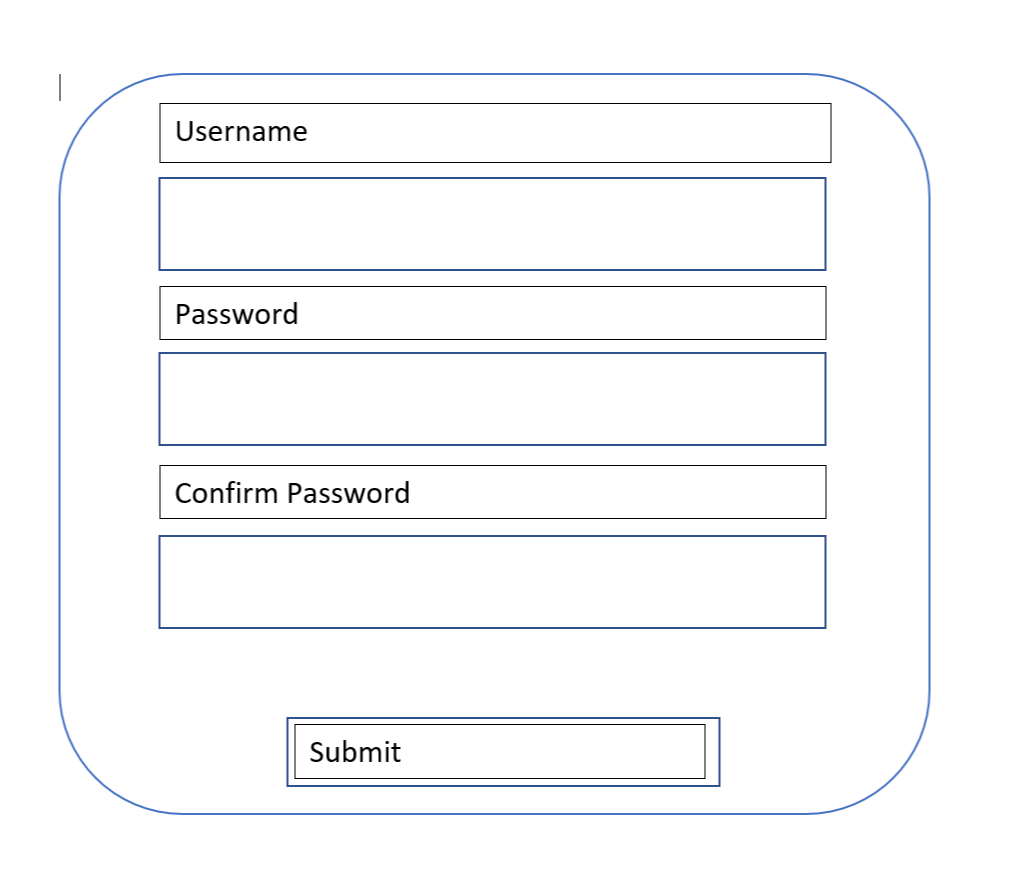
\includegraphics[width=\linewidth]{createaccount}
\end{minipage} \hfill

\subsection{Control Mechanisms}

The user will be able to select either a touch screen control or a keyboard control scheme. 
The player will be able to move left and right, the player will be able to move forward.
The direction will be relative to the players position as the camera direction will be random at the start of the game.
There will be a circular control function on the screen, slightly transparent so that it does not obstruct the players view.
This control will allow the player to control how the ball rolls.

\section{Game Mechanic}

\begin{minipage}{.9\textwidth}
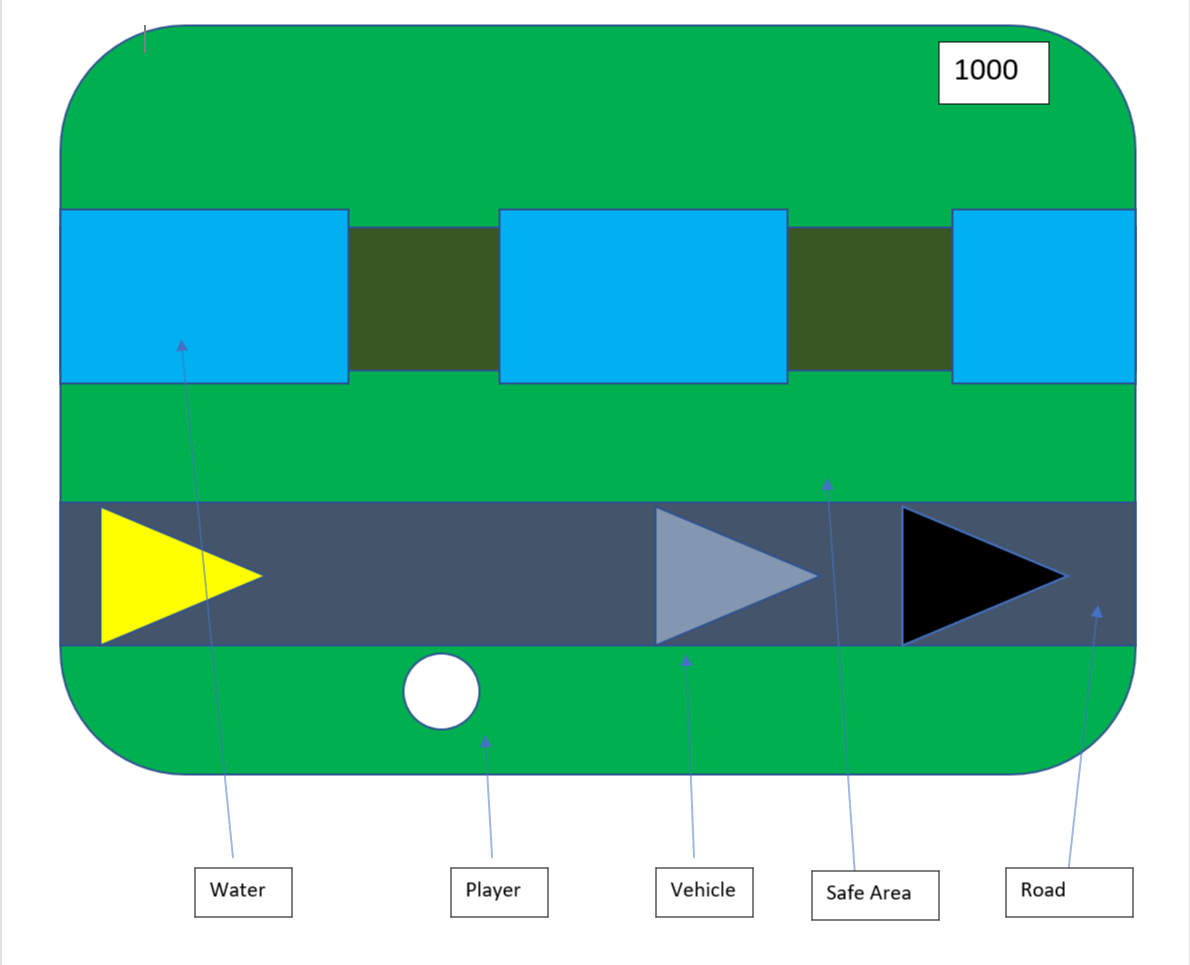
\includegraphics[width=\linewidth]{ingame}
\end{minipage} \hfill

\begin{itemize}
\item The player will choose between an easy mode, normal mode or hard mode, Difficulty will be increased based on this decision.
\item The game will start with a ball at a static position. The player will be able to move the ball, using the touch screen.
\item In front of the player random segments will be spawned, roads, water and safe segments where the player will be able to stop if needed.
\item Each of the roads will spawn vehicles at random intervals and travelling at various speeds to increase the games difficulty.
\item The player will gain points by crossing the roads and panels.
\item Roads are created procedurally during the game, the roads and safe segments are randomly generated, but the safe space will automatically created if 3 road segments are generated in a row, this means there will be no chance of generating 4 roads side by side.
\item The game has no end to the level, known as an infinite runner. The idea of the game is to  get the highest possible score.
\item The game will end when the ball comes in contact with a vehicle, if the ball falls in the water, or remains static until the progressing screen reaches the ball.
\end{itemize}

\section{System Compatibility}

The game will be compatible with any system windows UWP can run on. As it is a Unity project it could be compiled for many other systems, but for the moment I will stay with the systems that the project requires. The game will be designed to run on windows touch screen devices and windows Desktops.

\section{Hardware Functions Used}

The hardware being used will include a Touch screen device and use touch controls for the game, Keyboard controls will also be available for non touch screen devices.

\section{Conclusion}

\section{References and Sources}

16personalities.com. (2018). Might or Magic? A Study of Gamers’ Personality Types | 16Personalities. [online] Available at: https://www.16personalities.com/articles/might-or-magic-a-study-of-gamers-personality-types [Accessed 20 Sep. 2018]. \newline

Film.avclub.com. (2018). [online] Available at: https://film.avclub.com/the-king-of-kong-a-fistful-of-quarters-1798202980 [Accessed 18 Sep. 2018]. \newline


Eurogamer Interview with Shigeru Miyamoto and Takashi Tezuka, (2018). [video] Available at: https://www.youtube.com/watch?v=zRGRJRUWafY [Accessed 18 Sep. 2018].

Twin Galaxies. (2018). Billy Mitchells Donkey Kong and All Other Records Removed. [online] Available at: www.twingalaxies.com/ [Accessed 18 Sep. 2018]. \newline

En.wikipedia.org. (2018). Defender (1981 video game). [online] Available at: https://en.wikipedia.org/ [Accessed 18 Sep. 2018]. \newline

Kent, Steven (2001). "The Golden Age (Part 1: 1979–1980)". The Ultimate History of Video Games. Three Rivers Press. pp. 144–147. \newline

 "Top 100 Arcade Games: Top 20–6". Guinness World Records Gamer's Edition 2008. Guinness World Records. Guinness. \newline
 
 Kuchera, Ben (November 21, 2014). "Crossy Road has invented the 'endless Frogger,' and it's brilliant". Polygon. 
 https://www.polygon.com/2014/11/21/7260459/crossy-road-frogger \newline

\end{document}